\documentclass[english]{article}

\usepackage{graphicx}
\usepackage{grffile}
\usepackage[T1]{fontenc}
\usepackage{babel}

\author{
	Maree, Armand\\
	\texttt{12017800}
	\and
	Watt, Brenton\\
	\texttt{14032644}
	\and
	Meyers, Charl\\
	\texttt{14024633}
	\and
	Tom, Elton\\
	\texttt{13325095}
	\and
	Tswene, Kamogelo\\
	\texttt{12163555}
	\and
	Molefe, Keletso\\
	\texttt{14222583}
	\and
	Spazzoli, Lorenzo\\
	\texttt{13304862}
}

\title{Software Requirements Specification,\\
	Technology Neutral Process Design\\
	and\\
	Software Architecture Specification
}
\date{\today}
\graphicspath{{Pictures/}}
\begin{document}
	\maketitle
	\begin{figure}[!t]
		
\includegraphics[width=\linewidth]{up_logo.png}
	\end{figure}
	\pagenumbering{gobble}
	\newpage
	\tableofcontents
	\newpage
	\pagenumbering{arabic}
	
	\section{Introduction}
		\paragraph\indent
			In this document it would be specified how a system would be developed for the department of computer science at the University of Pretoria in order for them to replace their current, not so efficient Microsoft Office Excel spreadsheet, system with a more concurrent and reliable option.

	\section{Vision}
		\paragraph\indent
			The client requires a system that would allow them to retrieve and submit meta-data about academic papers published by the department of computer science at the University of Pretoria. Certain users would be able to create new papers and the project leader would then be able to control certain properties of the project, like the current progress of the paper. It should also have a web interface where changes can be made and also an Android app.

	\section{Background}
		\paragraph\indent
			 What lead to the project is the fact that that the client is facing a problem with the current system they are using.  The spreadsheet which does fulfill its task of storing details about user's publications, does not have a user friendly interface, and does not allow researchers to see any changes made to the system immediately, it is also not a concurrent system and is deemed less reliable.  The client wants a system that would improve the manner the users would be able to view their submissions and be able to modify the system to their liking, with changes immediately visible to researchers. Another aspect which lead to the development of a new system which would simplify the collaboration between the University of Pretoria users and users from other universities, is that instead of having a system which is local; a web interface could be used which is more accessible. The lack of ability to easily access previously entered user information data such as one’s username or contact details also was a factor that lead to this project, as it would be more convenient and efficient to have to have an interface that would for example have a drop down list of all the user information data on the system.

	
	\section{Architecture Requirements}
		\subsection{Access channel requirements}
			\paragraph\indent
				The system requires 2 interfaces:
			\begin{list}{$\bullet$}{\leftmargin=1.5cm \itemindent=0em}
				\item Web interface
				\item Android app (Could also be a mobile website)
			\end{list}

		\subsection{Quality requirements}
			\paragraph\indent
				The following quality aspects needs to be addressed:
			\begin{list}{$\bullet$}{\leftmargin=1.5cm \itemindent=0em}
				\item \textbf{Scalability:} Less a 100 users will use the system.
				\item \textbf{Security:} Passwords will be hashed with the SHA512 hashing algorithm.
				\item \textbf{Reliability:} An automatic partial dump backup will be done everyday at 03:00 and each back up will be kept for a week. On top of this a full dump will be done every 3 days and will be kept for 2 weeks. Alternatively the backup will be done by an external program. 
				\item \textbf{Audibility:} Every change should be logged and the person responsible for that log will be recorded. This will allow the administrators to track which users change what.
				\item \textbf{Maintainability:} Data that is deleted will only be moved to another database that might be a little slower. This will help alleviate some pressure off the main database.
				\item \textbf{Cost:} The total hours is estimated to be 120 at a cost of R500 per hour.
			\end{list}
			
		\subsection{Integration requirements}
			\paragraph\indent
				The system should allow universities to connect to each other using an API. This would allow them to collaborate on projects and also to track the papers that are being written. The Android app should also be able to connect to the server via the API.
			
			\paragraph\indent
				The protocol that will be used to transfer the data between the server and the clients will be the Hyper Text Transfer Protocol Secure (HTTPS). And the third parties that integrate with the system will access it either through the web interface, the mobile app or the provided API.
			
			\paragraph\indent
				Some quality requirements that have to be considered are:
			\begin{list}{$\bullet$}{\leftmargin=1.5cm \itemindent=0em}
				\item \textbf{Security:} The data that is sent over the Internet should be encrypted and it has been decided to use the Secure Socket Layer (SSL) encryption algorithm.
				\item \textbf{Reliability:} The reliability of the transfer of the data is dependent on the reliability of the internet connection.
			\end{list}
			
		\subsection{Architecture constraints}
			\paragraph\indent
			There are currently no architecture constraints that the client mentioned.
			

	\section{Functional requirements and application design}
		\subsection{Use case prioritization}
			\paragraph\indent
			\textbf{Critical:}
				\begin{list}{$\bullet$}{\leftmargin=1.5cm \itemindent=0em}
					\item There must be some web hosting server in order to be able to host a web interface, this interface will be the main access channel to the system as it makes it easier to access the system on a computer or non-Android device. If there is no web-server then there will be no web interface that can be accessed from research groups all over the country. This defeats the whole purpose of the system.
					\item The web interface needs to be accessible from the Internet preferably so that other research groups outside the University are able to access the system.
					\item The system needs to be able to save data in some way. If there is no possible way to store data then the system might as well not exist, because the purpose of the system is to store meta data about research papers.							
				\end{list}
			\paragraph\indent
			\textbf{Important:}
			\begin{list}{$\bullet$}{\leftmargin=1.5cm \itemindent=0em}				
				\item Users must be able to download a bibliography of papers released in a selected period.
				\item An Android app must be available that can access the system to make it easier to access the system on the go.			
				\item Users must create their user profile manually and will not be able to link the system with a web service in order to create their profile.
				\item No item should ever be deleted in the system. Everything is kept. Old unaccessed data may be archived but never deleted. There needs to be some sort of recovery or backup system that enables a user to restore accidentally deleted data.
				\item The system must be able to handle a max of at least 50 concurrent users as there is a possibility that at least 50 users may access the system all at once. There will also be an estimate of at least a 1000 users. The system must be able to handle that amount of users.
			\end{list}
			\paragraph\indent
			\textbf{Nice-to-have:}
			\begin{list}{$\bullet$}{\leftmargin=1.5cm \itemindent=0em}
				\item The system must be lightweight.
				\item The system must show the completion of a paper in percentage that a user specifies after editing the paper.
				\item The system may link with Google Calender to synchronize due dates and alerts for the paper a user is busy working on.
				\item The web interface can be designed to work on mobile phones for those who want to access the system on the go but do not have an Android device.
			\end{list}
		
		\subsection{Use case/Services contracts}
			\paragraph\indent
			\begin{list}{$\bullet$}{\leftmargin=1.5cm \itemindent=0em}
				\item\textbf{Use Case:} Add a paper.
				
				\textbf{Primary Actor:} Registered author or HOD.
				
				\textbf{Brief:} Only an author or head of department can add new papers.
				
				\textbf{Postconditions:}
				\begin{itemize}
					\item The article is saved to the database.
					\item All authors are notified of their new paper.
					\item The changes are logged.
					\item Paper is displayed.
				\end{itemize}
				
				\textbf{Triggers:} The user invokes the Add New Paper request.
				
				\textbf{Basic flow:}
				\begin{enumerate}
					\item Present the actor with a new paper form.
					\item Actor fill in the form and clicks submit.
					\item The data is sent to the server and added to the database and logs the event.
					\item Actor is presented with a success message.
					\item Paper is presented to the actor.
					\item Authors are notified.
				\end{enumerate}
				
				\item\textbf{Use Case:} Editing a paper.
				
				\textbf{Primary Actor:} Author of paper or HOD.
				
				\textbf{Brief:} Only an author involved with the paper or head of department can edit the paper.
				
				\textbf{Preconditions:}
					\begin{itemize}
						\item Author is presented with the paper in edit mode.
					\end{itemize}
				\newpage
				\textbf{Postconditions:}
					\begin{itemize}
						\item The article is saved to the database.
						\item All authors are notified of the changes.
						\item The changes are logged.
						\item Paper is displayed.
					\end{itemize}
					
				\textbf{Triggers:} The user invokes the Edit Paper request.
				
				\textbf{Basic flow:}
					\begin{enumerate}
						\item Present the actor with the paper in edit mode.
						\item Actor makes all desired changes and clicks submit.
						\item The data is sent to the server and added to the database and logs the event.
						\item Actor is presented with a success message.
						\item Paper is presented to the actor.
						\item Authors are notified.
					\end{enumerate}
					
					\item\textbf{Use Case:} Viewing a paper.
					
					\textbf{Primary Actor:} Author of paper or HOD.
					
					\textbf{Brief:} Only an author involved with the paper or head of department can view the paper.
					
					\textbf{Preconditions:}
					\begin{itemize}
						\item Author is presented with the paper in read-only mode.
					\end{itemize}
					
					\textbf{Triggers:} The user invokes the View Paper request.
					
					\textbf{Basic flow:}
					\begin{enumerate}
						\item Present the actor with the paper in read-only mode.
						\item When the actor is done viewing they simply navigate away. No changes or events has to be logged.
					\end{enumerate}
			\end{list}
			\paragraph\indent
			\textbf{Request and Results Data Structures:}
				See figure 1.
				\begin{figure}[!h]
					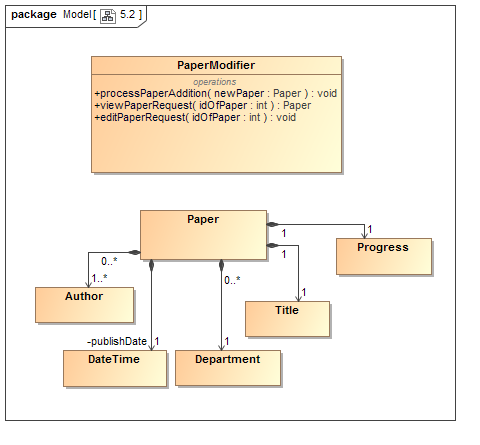
\includegraphics[width=\linewidth]{5.2.png}
					\caption{UML diagram for Request and Results Data Structure.}
				\end{figure}
				\clearpage
		\subsection{Required functionality}
			\begin{itemize}
				\item	Add a paper Use case: See figure 2
					\begin{figure}[!h]
						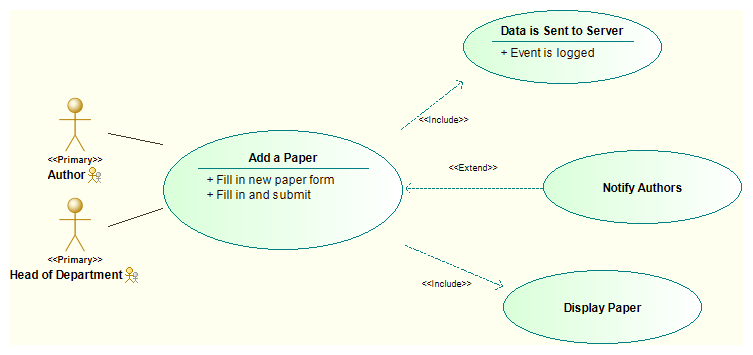
\includegraphics[width=\linewidth]{Add A Paper Use Case}
						\caption{Use case diagram for adding a paper}				
					\end{figure}
				\item   Edit a paper Use case: See figure 3
					\begin{figure}[!h]
						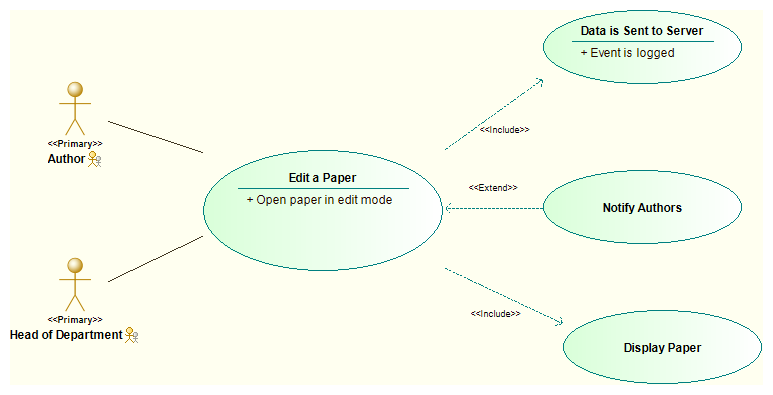
\includegraphics[width=\linewidth]{Edit a Paper Use Case}
						\caption{Use case diagram for editing a paper}				
					\end{figure}
				\item   View a paper Use case: See figure 4		
					\begin{figure}[!h]
						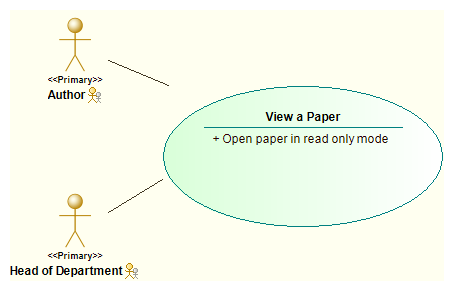
\includegraphics[width=\linewidth]{View a paper Use Case}
						\caption{Use case diagram for viewing a paper}
					\end{figure}									
			\end{itemize}
			\clearpage
		\subsection{Process specifications}
			\begin{itemize}
				\item Activity diagram to add a paper: See figure 5
					\begin{figure}[!h]
						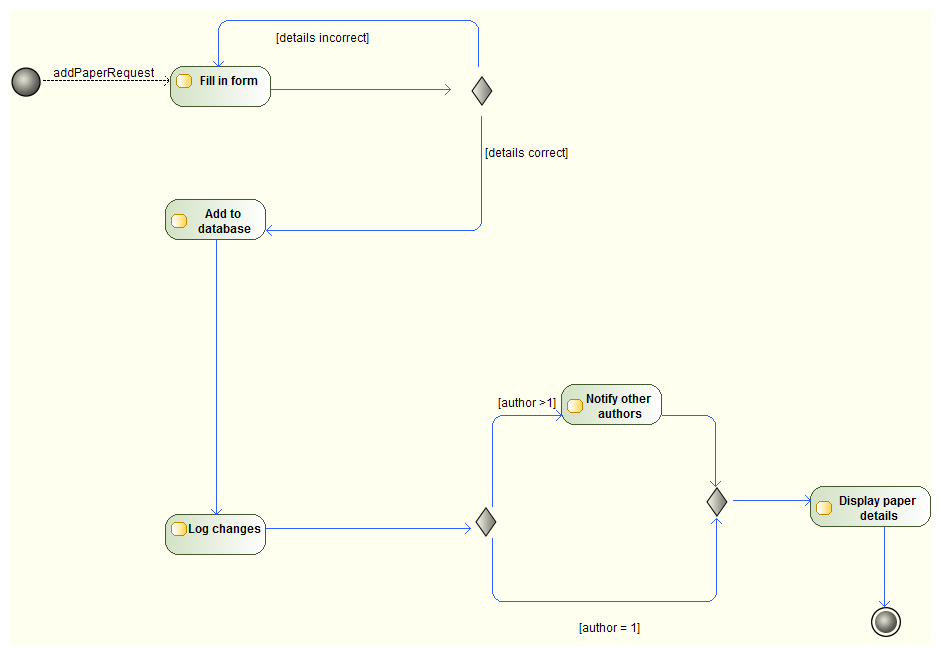
\includegraphics[width=\linewidth]{Activity diagram-Add a paper.png}
						\caption{Adding a paper to the database}
					\end{figure}
				\item Activity diagram to edit a paper: See figure 6
					\begin{figure}[!h]
						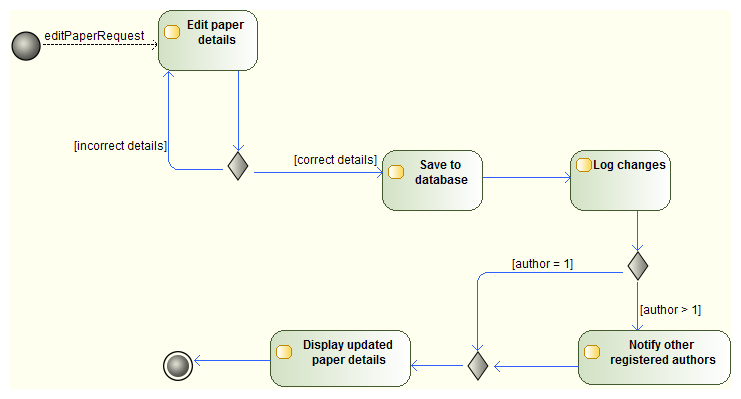
\includegraphics[width=\linewidth]{Activity diagram_Edit a paper.png}
						\caption{Editing a paper}
					\end{figure}
				\item Activity diagram to Login: See figure 7
						\begin{figure}[!h]
							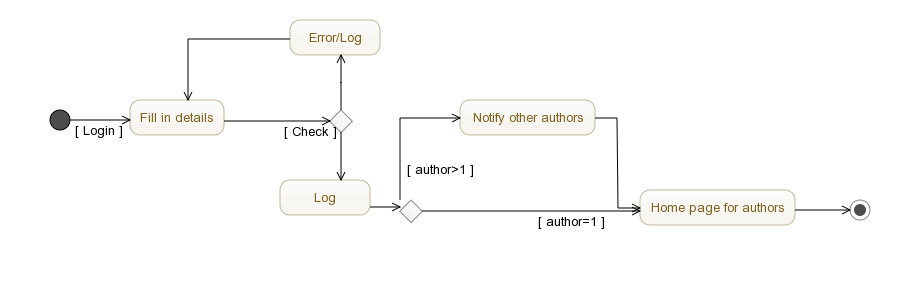
\includegraphics[width=\linewidth]{Activity.Login.jpg}
							\caption{Login to system}
						\end{figure}
				\item Activity diagram to Request document details: See figure 8
					\begin{figure}[!h]
						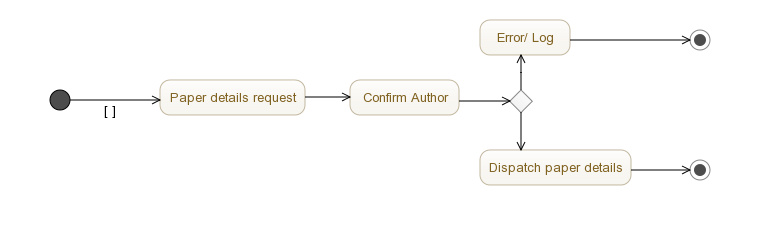
\includegraphics[width=\linewidth]{Pictures/Request.Paper.jpg}
						\caption{Request paper details}
					\end{figure}	
			\end{itemize}
			\clearpage
		\subsection{Domain Model}
			\begin{list}{$\bullet$}{\leftmargin=1.5cm \itemindent=0em}
				\item Domain Model of the system: See figure 9
					\begin{figure}[h!]
						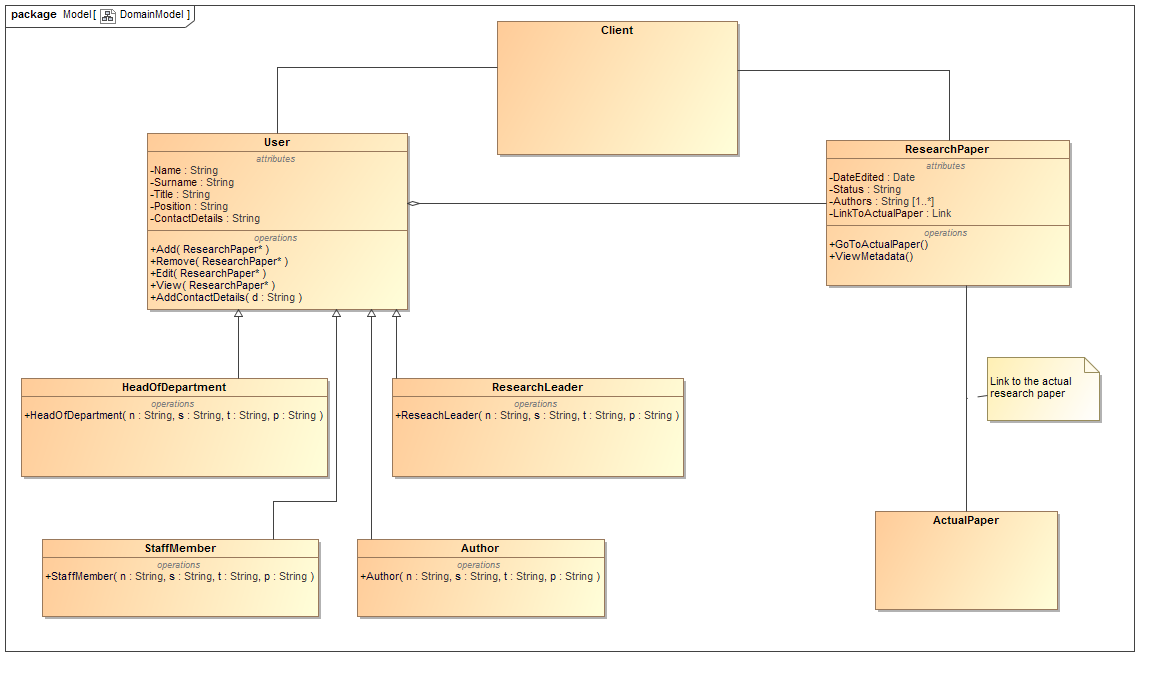
\includegraphics[width=\linewidth]{Pictures/5-5.png}
						\caption{Domain Model}
					\end{figure}
			\end{list}
			\clearpage
	\section{Software Architecture Documentation}
		\subsection{Architecture requirements}

			\subsubsection{Architectural scope}
			
				\paragraph\indent
				The architectural responsibilities that need to be handled by the software architecture are as follows:
				\begin{list}{$\bullet$}{\leftmargin=1.5cm \itemindent=0em}
					\item A main database that will store the papers that are added.
					\item A secondary database (separate from the first) that will act as the backup database where the partial and complete dumps will be stored.
					\item An infrastructure that will allow for notification to contributing authors that changes have been made to a paper they collaborated on, this infrastructure will also create a log of changes and who made them so that there is accountability.
					\item An infrastructure that will allow the users of the system to create and add papers to the database mentioned above as well as being able to edit and view them later.
					\item A mobile version of the above previously mentioned infrastructure must also exist. 
				\end{list}
			\subsubsection{Quality requirements}
				\paragraph\indent
				In order of importance our quality requirements are:
				\begin{list}{$\bullet$}{\leftmargin=1.5cm \itemindent=0em}
					\item \textbf{Reliability:} This is highly important as this might be the only place research could be backed up to, therefore, the system needs to be reliable. Reliability in this system is measured against the effectiveness of the backup measures in place as well as the system be available on demand. This will be achieved by the an automatic partial dump backup occurring daily in the early hours of the morning and a full dump once every 3 days.
					\newline \textbf{Strategy used:}
					\newline Maintain Backup, Checkpoint Rollback
					\newline \textbf{Design Patterns:} 
					\newline Memento design pattern may be used to roll back database to previous state in the event of some type of failure. Visitor Pattern will be used for creating the partial and full backup dumps.
					\item \textbf{Security:} The system needs to be secure from anyone who does not (or should not) have permission to use it, therefore passwords will be secured using the SHA512 hashing algorithm.
					\newline \textbf{Strategy used:}
					\newline Limit access strategy, by using Authentication and Authorization strategies.
					\newline \textbf{Design Patterns:}
					\newline Authenticator and Authorization Enforcer Patterns used for managing and delegating the authorizing and authenticating processes of users.
					\item \textbf{Audibility:} This is measured in terms of is every change noted and logged somewhere. This will be done through means of recording, when a change is made, the system will log the change as well as the user name that submitted the change, therefore everyone will be held accountable.
					\newline \textbf{Strategy used:}
					\newline No specific strategy tactic will be used for this
					\newline \textbf{Design Patterns:}
					\newline No specific design pattern will be used for this				
					\item \textbf{Scalability:} There will not be a huge amount of users making use of the system but it is important that if need be every user can make use of the system concurrently. This will be achieved by implementing the system in such a way that it is multi-threaded. In terms of two users trying work on the same documents meta-data simultaneously, when a user tries to upload an edited version of the documents meta-data, if the version on the system differs from the original document then the user will be alerted that there is a synchronization error and he should update the local version of the document and add the changes. This will avoid data corruption.
					\newline \textbf{Strategy used:}
					\newline Thread pooling and Use Concurrencies strategies
					\newline \textbf{Design Patterns:}
					\newline No specific design pattern will be used for this
					\item \textbf{Maintainability:} Measured against how effectively the system chooses to relocate data due to age. When data has been on the system for a predetermined length of time, it will be moved from the main system and relocated to a different (most likely slower) database and if a user wishes to make use of it again it can be called from there.
					\newline \textbf{Strategy used:}
					\newline No specific strategy tactic will be used
					\newline \textbf{Design Patterns:}
					\newline Visitor design pattern will be used for relocating data to a different database
				\end{list}
			
			\subsubsection{Integration and access channel requirements}
				\paragraph\indent
				The Integration and access channel requirements are:
				\begin{list}{$\bullet$}{\leftmargin=1.5cm \itemindent=0em}
					\item \textbf{Centre of integration:} This will be the main Server, probably an HTTP/HTTPS Server that will be feeding data to other sub-parts of the system. The main Server will be directly connected to all the Databases. It will be the source of data. To prevent anyone one from connecting to the Server, a password will have to be provided, checks will be done to check if the sub-part of the System is authorized, this could be anyone from outside who will be trying to connect to the server, e.g the Android Application, Client as (Website) and windows application.
					\item \textbf{sub-parts of the system:} This will be anyone who will be trying to gain access to the Server. The sub-part of the system will have to prove to the server that it is authorized to gain access to the information held by the server. Login details and passwords will be provided to the server to allow access.
					\item \textbf{Protocols to be used(Access channels):} HTTP/HTTPS will be used,  the sub-parts of the system will have to go through the HTTP/HTTPS to gain access to the server. If the subsystem fails to prove to the Server through HTTPS/HTTP it will not be allowed access to the Server's data.
					\item \textbf{Gaining of data from Server:} The server will contain an API that will allow the sub-parts of the system to gain access of the data through function calls, and authentication will be taking during the communication of the Server and the client(sub-part of the system). To make the security reliable, authentication will have to take place regularly.
				\end{list}
			
			\subsubsection{Architectural constraints}
				\paragraph\indent
				Architectural contraints are as follows:
				\begin{list}{$\bullet$}{\leftmargin=1.5cm \itemindent=0em}
					\item \textbf{particular technologies:}For web development we have to use css, html and javascript.
					\item \textbf{Operating System:} The System must be available on Web Browsers and on Android devices. The system should run in any Operating System(for Web Based) and Should run on android operating system for android(mobile device).
				\end{list}
			
			
		\subsection{Architectural patterns or styles}
			\paragraph\indent
			Architectural patterns are usually seen as commonalities at a higher level than design patterns. An Architectural pattern such as PAC (Presentation-Abstraction-Control), MVP (Model View Presenter), or the MVC (Model View Control) can be used to mechanisms of a system. MVC would be the preferred Architecture as it allows a user to enter input or perform a state query after then manipulation takes place and in return the result would be displayed for the user to see.
			
			\paragraph\indent
			MVC Architectural pattern:
			\begin{list}{$\bullet$}{\leftmargin=1.5cm \itemindent=0em}
				\item Model � Here the data that was entered by the user would be internally processed.
				\item View - This is the interface that would allow the user to enter data/information into the system and as a result the reflected changes would be seen by the user.
				\item Controller � User entered data would be received by the controller and all other application flow would be managed by the controller.
			\end{list}
			
			\paragraph\indent
			Layering would consist of three levels - Client, Application Logic, and the Database Management System, as in the figure below:
			\begin{figure}[!h]
				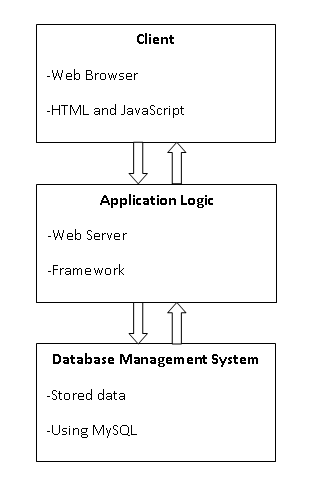
\includegraphics[width=\linewidth]{Pictures/Layering design.png}
				\caption{Layering of the system}
			\end{figure}
			
			
		\subsection{Architectural tactics or strategies}
			\paragraph{Performance}\indent
			To better manage resource intensive tasks thread pooling will be used. There will be an object that receives all tasks and allocates them to a specified thread when a thread becomes available.
			
			\paragraph{Exception handling}\indent
			Exceptions should be dealt with as soon as and as best as possible, but since it cannot be afforded that the system crashes there should be some form of "last resort" that attempts to deal with unhandled exceptions in such a way that the system as a whole keeps functioning.
			
			\paragraph{Passive Redundancy}\indent
			There will be 2 databases that will both contain all the information. This will increase the reliability of the system by having a back up database that can take over at any point when the primary database fails. This will be transparent to the user.
			
			\paragraph{Transactions}\indent
			Changes to the database will be done in transactions that will allow any changes to be rolled back to a checkpoint should an error occur. This will cause atomicity in the system and increase reliability.
			
			\paragraph{Security}\indent
			Encryption to increase security HTTPS protocols will be used to transmit data and all private information (like passwords) will be hashed using the SHA512 hashing algorithm.
			
			\paragraph{Integrability}\indent
			In order to increase integrability a modular approach will be taken when implementing the system by using dependency injection as far as possible.
			
		\subsection{Use of reference architectures and frameworks}
			\paragraph\indent 
			\begin{itemize}
				\item Bootstrap for styling the Web interface of the system. Will be used for alignment of the elements of the web interface, any alignment for tables (if any) and responsive design so that the  web interface can be viewed on mobile devices.
				\item AngularJS will be used for the front end of the website along with bootstrap by using UI Bootstrap. For example, it will be used for DOM manipulation and data-binding can be used to send data to the server. Most notable and obvious use is when a new user creates an account, AngularJS will handle and send the data entered by the user to the server.
				\item PhoneGap (renamed to Apache Cordova, we will use PhoneGap in this document) will be used as a wrapper for the above website in mobile form. Meaning the web interface will be used and PhoneGap will create a hybrid Android app that communicates with the server and only acts as an interface to enter data.
				\item Ionic framework will be used together with AngularJS and PhoneGap and replace Bootstrap for the hybrid android app. ionic makes better and responsive apps when used with PhoneGap and requires angularJs. The reason it will replace Bootstrap for the mobile app is because Bootstrap and Ionic do not play well because of name conflicts.
				\item Spring framework will be mainly used for dependancy injection on the server side of the system. The MVC nature of Spring will also be of good use for the needs of the system. Spring is also some kind of wrapper for Java EE.
				\item Java EE can be seen as a reference architecture that supports scalability, MVC and dependancy injection. All are needed to be implemented in the CS Research System.
			\end{itemize}
			
		\subsection{Access and integration channels}
			\paragraph\indent
			The different access channels that will enable users to use the system are a web interface, which can be accessed from either a computer or mobile phone as well as a mobile app, preferably an Android app.
			
			\paragraph\indent
			The integration channel through which our system will integrate with external systems is a database, which will be able to store data about the users as well as the details of the papers that the users contribute to. The database organises large amounts of data, that is then easier to access, manage and update. An API will also be used so that users from different universities can connect to the system and contribute to any project that they are working on.

			\paragraph\indent
			The protocol that will be used is the Hypertext Transfer Protocol Secure (HTTPS), because it enables for data to be sent securely through to the server and also because the privacy and integrity of the data that is sent between the server and the system is protected, which is regarded as important as the content of the system should be safe from unauthorized users.

			\paragraph\indent
			For the integration channel, the technology that will be used for the database is MySql, a database used on the web and that most people are familiar with. It is also easy to use, reliable, fast and it can cater for large applications.

		\subsection{Technologies}
			\paragraph\indent
			Technologies used will be MySQL for the database , it is very light weight and will have sufficient access control for the given product. The server will be a mix of PHP and Java, both will connect to MySQL , the Java will be the host for the android connection and the PHP will handle requests from the web interface.
	\section{Open Issues}	
		\paragraph\indent	
		There are currently no open issues.
\end{document}
